\documentclass[11pt,a4paper]{article}
\usepackage[utf8]{inputenc}
\usepackage{amsmath}
\usepackage{amsfonts}
\usepackage{graphicx}

\usepackage[table,xcdraw]{xcolor}

\usepackage{caption}
\usepackage{subcaption}
\usepackage{float} % para que floten las imagenes o algo asi...
\usepackage{wallpaper} %paquete para usar una imagen como encabezado!
\usepackage{hyperref} %para usar hypervinculos 
\usepackage[export]{adjustbox} %para usar marcos en imagenes
\usepackage{eurosym} % para el euro
\usepackage{transparent} %para las marcas de agua
\usepackage{eso-pic}  %para las marcas de agua
\definecolor{azul_marcos}{RGB}{0,128,159} %defino el color azul de los marcos
\usepackage{sectsty} %esto es para cambiar el color de las fuentes creo
\renewcommand{\familydefault}{\sfdefault} % cambiamos la fuente a una sans
\sectionfont{\color{azul_marcos}}  % sets colour of sections
\subsectionfont{\color{azul_marcos}}  % sets colour of sections
\usepackage{pdfpages} %para insertar pdfs
\usepackage{amssymb}
\usepackage{pstcol} % para color
\usepackage{pst-node} % para diagramas
\usepackage{pst-plot} % para representacion de dat
\usepackage[spanish]{babel}
\addto\captionsspanish{\renewcommand\chaptername{Bloque}}
%\usepackage[total={18cm,21cm},top=2cm, left=2cm]{geometry}
\usepackage{anysize}
\pagestyle{plain}
%\markboth{left head}{right head}
%\markright{Guía de impresión FlexiSMART}
\marginsize{3cm}{2cm}{2.5cm}{1cm}
\title{FlexiSMART printing guide}
\date{}

%configuracion de la marca de agua
\AddToShipoutPicture{
    \put(0,0){
        \parbox[b][\paperheight]{\paperwidth}{%
            \vfill
            \centering
            {\transparent{0.2}
\includegraphics[scale=1.25]{FOTOS/logofff}}%
            \vfill
        }
    }
}

\begin{document}
\ULCornerWallPaper{1}{FOTOS/header}
\LLCornerWallPaper{1}{FOTOS/footer}
%\maketitle
%\tableofcontents

\includepdf{PDF/EN_PORTADA.pdf}
\section{What is FlexiSMART?}FlexiSMART is a filament for 3D FFF/FDM printing made from thermoplastic elastomeric polymers (TPE) with chemical additives to make it easier to print for most 3D printers of the market.
\\\\
FlexiSMART is flexible and it gets its shape back when you fold it, twist it or stretch it.

\section{Why use a FlexiSMART?}
FlexiSMART lets you enter a new world of possibilities thanks to the flexible nature of the filament. From now on you can print objects you couldn’t before with a rigid filament: cases for Smartphone, tablets, slippers, templates, RC wheels, prosthesis, silent blocks, gears that need certain adaptability, and in general, any object you can think of and for which you can find a use.
\\\\
FlexiSMART has been design to be easily printed.
\begin{itemize}
\item It has a certain rigidness so that it can be printed by most direct extruders making none or few modifications.
\item Adherence is excellent. You can print it even without a heated bed.
\item Resistance is very high, for which the printed parts won’t get degraded quickly.
\item It’s the flexible filament with the most attractive prices in Europe.
\end{itemize}

\section{Data sheet and printing parameters}

\begin{table}[H]
\centering
\caption*{Data sheet}
\begin{tabular}{|
>{\columncolor[HTML]{FFFFFF}}l |
>{\columncolor[HTML]{FFFFFF}}c |}
\hline
\multicolumn{1}{|c|}{\cellcolor[HTML]{FFFFFF}\textbf{Material}}   & FlexiSMART (TPE)   \\ \hline
\textbf{Colors available}              & 11                 \\ \hline
\textbf{Formats available}             & 1kg, 250gr         \\ \hline
\textbf{Heat deflection temperature} & 90ºC               \\ \hline
\textbf{Melting Point}            & 160ºC              \\ \hline
\textbf{Decomposition temperature}    & \textgreater 240ºC \\ \hline
\textbf{Density}                         & 0.96 gr / cm3      \\ \hline
\textbf{Ultimate elongation}              & 600\%              \\ \hline
\end{tabular}
\end{table}
\begin{table}[H]
\centering
\caption*{Printing parameters recommended using a nozzle of 0.4 mm}
\begin{tabular}{|
>{\columncolor[HTML]{FFFFFF}}l |
>{\columncolor[HTML]{FFFFFF}}c |}
\hline
\multicolumn{1}{|c|}{\cellcolor[HTML]{FFFFFF}\textbf{Recommended printing temperature}} & 195º-220º              \\ \hline
\textbf{Recommended printing speed}                         & 20-60mm/s              \\ \hline
\textbf{Heated bed temperature}                                  & \textgreater 18º (it doesn’t need a heated bed)        \\ \hline
\textbf{Optimal layer height}                                      & 0.2 mm                 \\ \hline
\textbf{Perimeters}                                                 & 3                      \\ \hline
\textbf{Top solid layers}                                           & 5                      \\ \hline
\textbf{Retraction}                                                 & Deactivated or reduced \\ \hline
\end{tabular}
\end{table}

You can download our full printing profiles from the principal lamination programs (Cura, Slic3r y SImplify3D) from our web page:
\\\\
\centerline{ {\huge \url{www.fffworld.com/documentation} } }
\\\\
Optimal parameters will depend on the 3D printer you use, however, they’re good parameters to use as a starting point. With a few prints you’ll be able to find the limits and the perfect setting for your machine.
\section{Problems and solutions}
	\subsection{Problems extruding FlexiSMART}
The main challenge when printing FlexiSMART and other flexible filaments derives from the nature of the material itself since, by being flexible, it can’t be pushed as easily as rigid materials, in the same way you can’t push a rope.
\\\\
The problem arises when there are gaps on certain parts of the extruder, particularly, between the drive-gear (the dentate wheel that pushes the filament) and the hole through which the filament accesses the hot-end (metallic point that melts the filament).
\\\\
When this space is big enough the filament tends to get out of its route and make a knot that ends up poking through a side of the extruder, as can be seen on the image.
\begin{figure}[H]
\centering
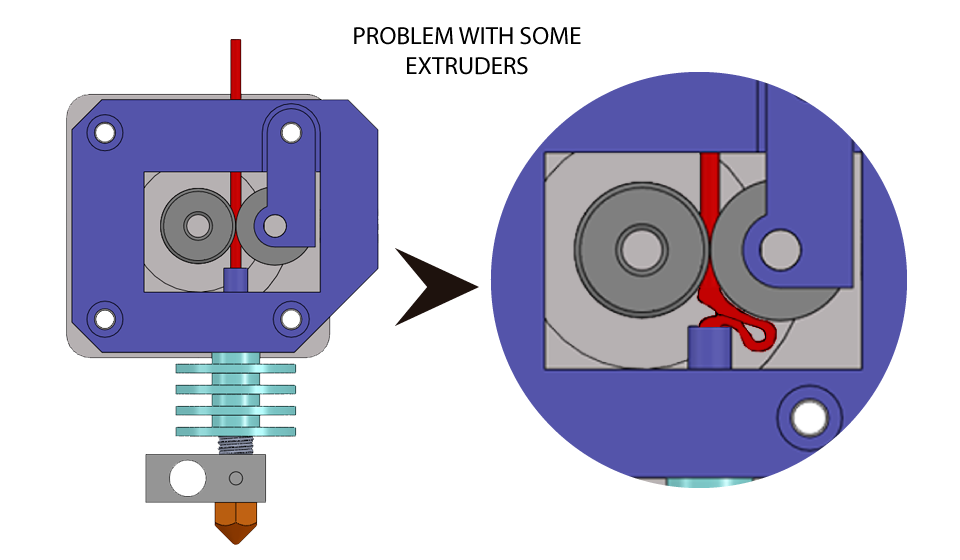
\includegraphics[width=0.5\textwidth,cfbox=azul_marcos 4pt 0pt]{FOTOS/NUDOS1}
\caption*{NON-optimized extruder for printing flexible filaments}
\end{figure}
This problem is bigger when using the 1.75 mm filament since by having less section is even more given to stray from its route.
\\\\
The speed of extrusion is determinant for the appearance of this problem. If the extruder tries to push the filament to the maximum speed an upwards pressure is created that makes the filament stray from its natural route. Therefore the general recommendation is to start printing at a slow or very slow speed and increase it until you reach the maximum speed your extruder can stand. The size of the nozzle also affects the maximum limit speed for the bigger this is the more melted material can be extruded per unit of time, and therefore, higher will be the velocity at which it can be done.
\\\\
The extruders designed to use flexible filaments minimize gaps stopping the filament from poking out and they incorporate a system of double drive-gear to channel with precision the filament and completely avoid the mentioned problem at the same time they allow to increase the printing speed.
\begin{figure}[H]
\centering
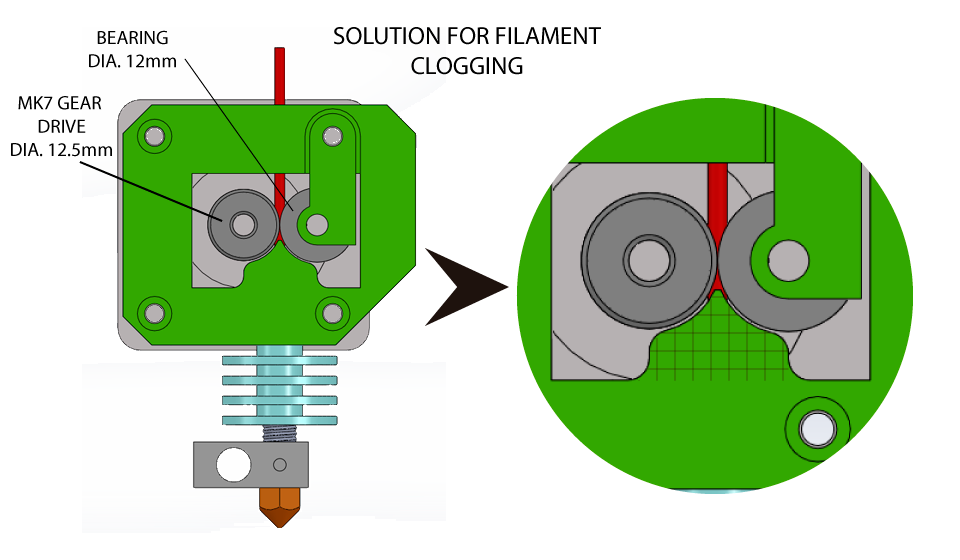
\includegraphics[width=0.5\textwidth,cfbox=azul_marcos 4pt 0pt]{FOTOS/NUDOS2}
\caption*{Optimized extruder for printing flexible filaments}
\end{figure}
\emph{FlexiSMART has been designed thinking of these problems and it has a rigidity superior to other flexible filaments to help reduce them.}
\\\\
However, on extruders that aren’t designed to use elastic materials these problems it may appear.
	\subsection{Preparing the extruder to print FlexiSMART}If you’re having any of the problems previously mentioned you probably have to adapt or replace your extruder. In this sense there are some options that we detail below.
		\subsubsection{Modify your extruder}
Sometimes it’s possible to use FlexiSMART on non-optimized extruders making some modifications on the extruder itself.
\\\\
If you’re having trouble printing FlexiSMART we suggest that you follow the following advices, exposed by complexity order.
			\paragraph{File the conduct through which the filament accesses the hot-end}\mbox{}\\\\
If you use an extruder with a plastic body, as the printable extruders, we recommend that you try the following. 
\\\\
Slightly file the edges of the hole right under the drive-hear, a hole through which the filament is channeled to the hot-end. This allows to avoid friction and hitches that may provoke the previously described knots. 
\\\\
It might be necessary to dismount part of the extruder to make this operation.
			\paragraph{Insert Teflon tube in the extruder}\mbox{}\\\\
A second option, more complicated but more effective, is to insert a Teflon tube (PTFE) in the mentioned hole. This technique also allows to reduce the space with the drive-gear since said tube can be placed very close to that one. You can even modify the entry to the Teflon tube to adapt it to the form of the drive-gear leaving a minimum space.
\\\\
In general this technique implies to drill the extruder to allow insertion of the mentioned Teflon tube. Here you can see some images of the result:
\begin{figure}[H]
    \centering
    \begin{subfigure}[b]{0.3\textwidth}
        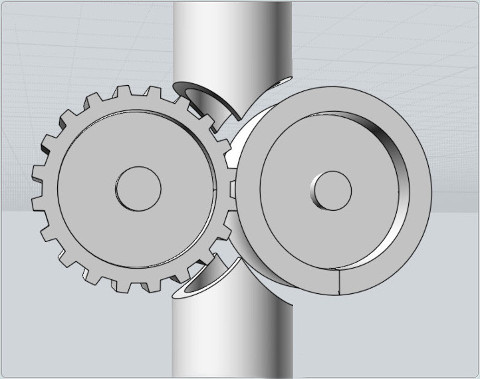
\includegraphics[width=\textwidth,cfbox=azul_marcos 4pt 0pt]{FOTOS/TEFLON1}
    \end{subfigure}
    ~ %add desired spacing between images, e. g. ~, \quad, \qquad, \hfill etc. 
      %(or a blank line to force the subfigure onto a new line)
    \begin{subfigure}[b]{0.3\textwidth}
        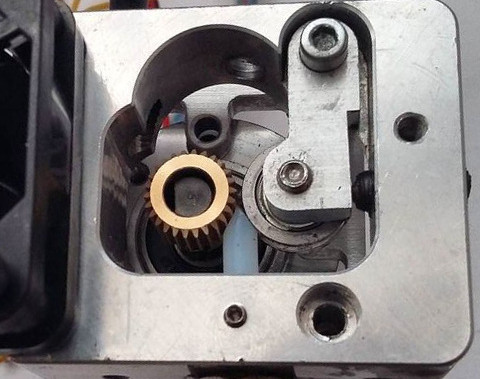
\includegraphics[width=\textwidth,cfbox=azul_marcos 4pt 0pt]{FOTOS/TEFLON2}
    \end{subfigure}
    ~ %add desired spacing between images, e. g. ~, \quad, \qquad, \hfill etc. 
    %(or a blank line to force the subfigure onto a new line)
    \begin{subfigure}[b]{0.3\textwidth}
        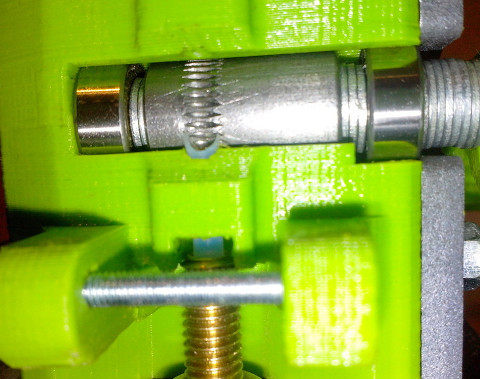
\includegraphics[width=\textwidth,cfbox=azul_marcos 4pt 0pt]{FOTOS/TEFLON3}
    \end{subfigure}
    \caption*{PTFE (Teflon) tube insertions}
\end{figure}
			\paragraph{Print a guide for the filament and put it in the extruder}\mbox{}\\\\
The third choice is to print a part that works as a guide for the filament and place it under the drive-gear. These parts usually have a triangular shape and should be designed respecting the dimension of each extruder.
\\\\
In the internet, in sites like \url{www.thingiverse.com}, you can download this type of adapters for some of the most usual extruders. However, this is a simple design that those with knowledge of 3D printing could easily create from scratch.In the internet, in sites like www.thingiverse.com, you can download this type of adapters for some of the most usual extruders. However, this is a simple design that those with knowledge of 3D printing could easily create from scratch.
\begin{figure}[H]
    \centering
    \begin{subfigure}[b]{0.5\textwidth}
        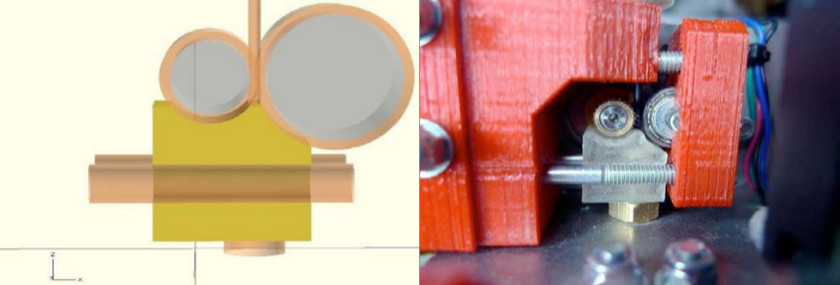
\includegraphics[width=\textwidth,cfbox=azul_marcos 4pt 0pt]{FOTOS/GUIA1}
    \end{subfigure}
    ~ %add desired spacing between images, e. g. ~, \quad, \qquad, \hfill etc. 
      %(or a blank line to force the subfigure onto a new line)
    \begin{subfigure}[b]{0.5\textwidth}
        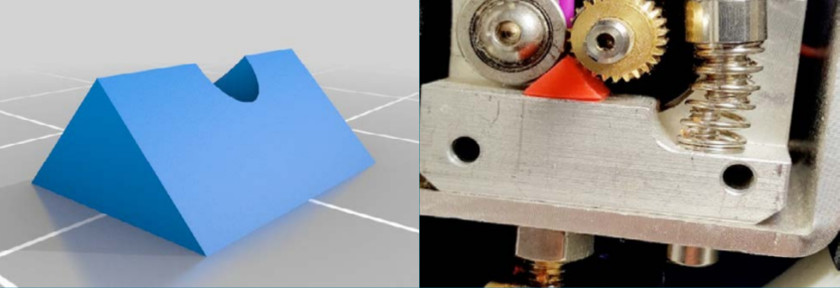
\includegraphics[width=\textwidth,cfbox=azul_marcos 4pt 0pt]{FOTOS/GUIA2}
    \end{subfigure}
    ~ %add desired spacing between images, e. g. ~, \quad, \qquad, \hfill etc. 
    %(or a blank line to force the subfigure onto a new line)
    \begin{subfigure}[b]{0.5\textwidth}
        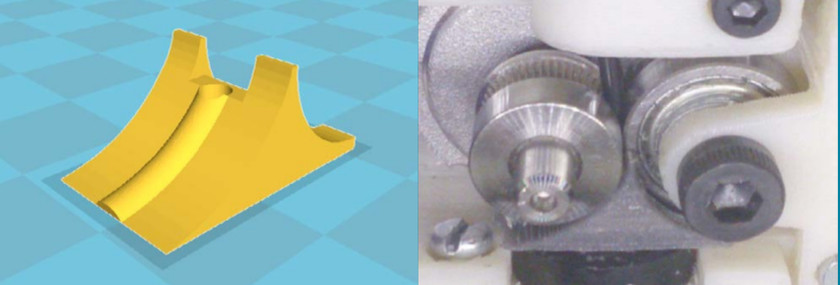
\includegraphics[width=\textwidth,cfbox=azul_marcos 4pt 0pt]{FOTOS/GUIA3}
    \end{subfigure}
    \caption*{Printable filament guides}
\end{figure}	

	\paragraph{Adjusting the pressure of the drive-gear over the filament}\mbox{}\\\\
This being a flexible material it’s particularly important that the pressure of the mechanism that pushes the filament towards the hot-end not be excessive. In the rigid filaments an excess of pressure will produce small notches in its surface but in the case of FlexiSMART an excessive pressure disfigures the section of the filament giving it an oval shape that makes it be more prone to clog the extruder.
\\\\
The extruders designed for the printing of flexible filaments consider this and have a mechanism to regulate the pressure of the tractor mechanism. If your extruder allows to regulate such pressure we recommend that you adjust it when using FlexiSMART. The adequate pressure will be the minimum necessary that allows the extruder to move the filament.
\\\\
If your extruder doesn’t have a mechanism to regulate the pressure you can still reduce it by changing the spring or reducing the possible route by placing a wedge on the right spot. As an example we show an image on how to reduce pressure in an extruder that is not ready for it:
\begin{figure}[H]
\centering
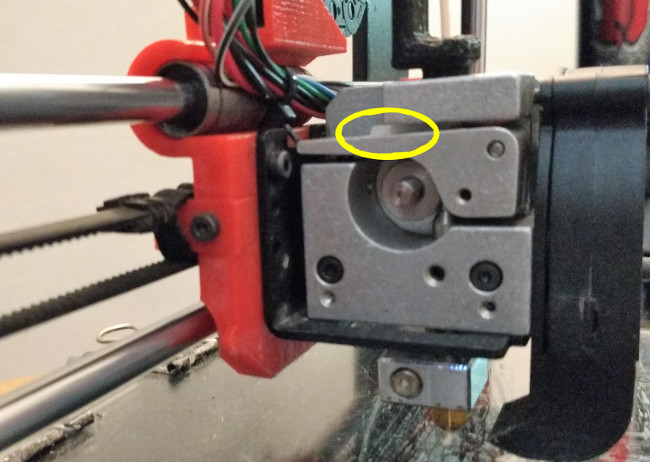
\includegraphics[width=0.5\textwidth,cfbox=azul_marcos 4pt 0pt]{FOTOS/SOLUCION1}
\caption*{HeatCore Extruder. BQ Hephestos and BQ Witbox}
\end{figure}
			\paragraph{Adding tension between the reel and the extruder}\mbox{}\\\\
It’s been proved that in some models of printers it’s convenient that when using flexible filament there be some tension between the reel and the extruder in a way that the filament isn’t left hanging.
\\\\
To get this you can try to stop the reel so that the extruder has to pull lightly from the filament to untangle it. You can also place a similar accessory to the one from the photograph to reach the same target.
\begin{figure}[H]
\centering
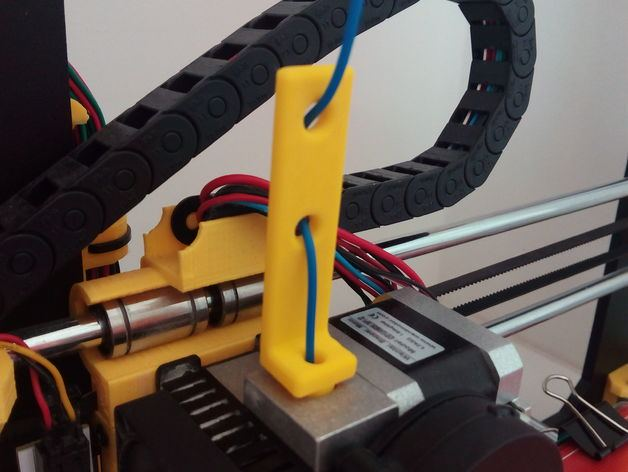
\includegraphics[width=0.5\textwidth,cfbox=azul_marcos 4pt 0pt]{FOTOS/SOLUCION2}
\caption*{Designed for BQ Unibody and BQ Hephestos extruder}
\end{figure}
		\subsubsection{Replace your extruder with an optimized one}
Nowadays flexible filaments have become popular to the point where it’s hard for a last generation printer not to be prepared to print them.
\\\\
Besides, many designers have created printable extruders capable of printing FlexiSMART and other filaments. These extruders can be downloaded from pages like Thingiverse to be printed and assembled at home.
\\\\
They’re also every time more the commercial extruders prepared to print flexible filaments that may be acquired and mounted on our printers.
			\paragraph{DIY printable extruders}
\mbox{}\\\\
Some of these extruders are designed from scratch and others are modifications made over existing designs. Here we present a non-exhaustive list of extruder designs that can downloaded from the internet. Following each link you could find the complete list of components as well as montage instructions and comments from other users.
\\\\
The hot-end you install on your extruder must have a Teflon tube (PTFE) inside to avoid frictions and so that FlexiSMART can be printed correctly. FlexiSMART has been successfully tested on the following hot-ends\footnote{You must keep into account that said tests have been made with original hot-ends and we can’t guarantee the result on imitations of such.}:
\begin{itemize}
\item J-Head MKV-B
\item Budassnozzle V1.3
\item E3D v6
\item Leonnozzle V2
\end{itemize}
Depending on what printer you use, some of these extruders will be easier to install given that they might replace the original extruder of the machine.
\begin{figure}[H]
    \centering
    \begin{subfigure}[b]{0.4\textwidth}
        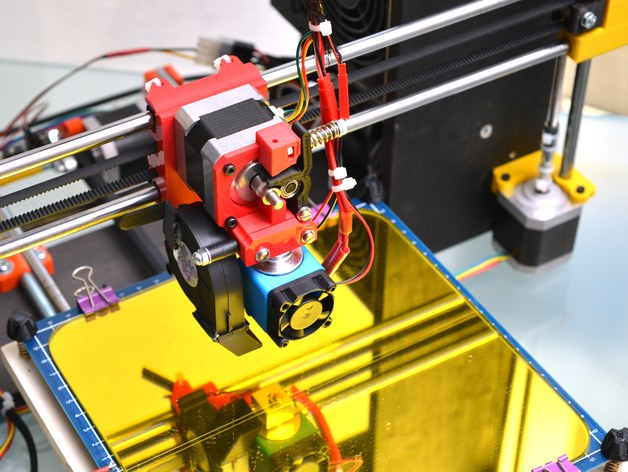
\includegraphics[width=\textwidth,cfbox=azul_marcos 4pt 0pt]{FOTOS/EXTRUSOR1}
		\caption*{\href{http://www.thingiverse.com/thing:147705}{{\footnotesize Direct-drive hinged extruder for E3D/J-Head hot-end (Prusa i3) by ffleury}}}
    \end{subfigure}
    ~ \qquad%add desired spacing between images, e. g. ~, \quad, \qquad, \hfill etc. 
      %(or a blank line to force the subfigure onto a new line)
    \begin{subfigure}[b]{0.4\textwidth}
        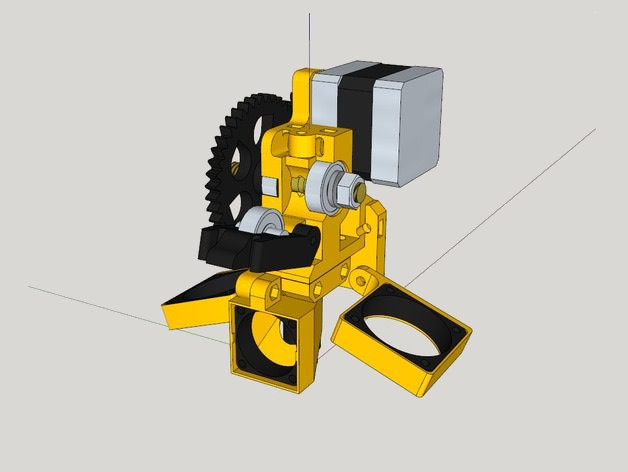
\includegraphics[width=\textwidth,cfbox=azul_marcos 4pt 0pt]{FOTOS/EXTRUSOR2}
		\caption*{\href{http://www.thingiverse.com/thing:512338}{{\footnotesize Wade L3K Extruder (prusa I3) compatible filament flexible By Skarab}}}
    \end{subfigure}
\end{figure}
\begin{figure}[H]
    \centering
    ~ %add desired spacing between images, e. g. ~, \quad, \qquad, \hfill etc. 
    %(or a blank line to force the subfigure onto a new line)
    \begin{subfigure}[b]{0.4\textwidth}
        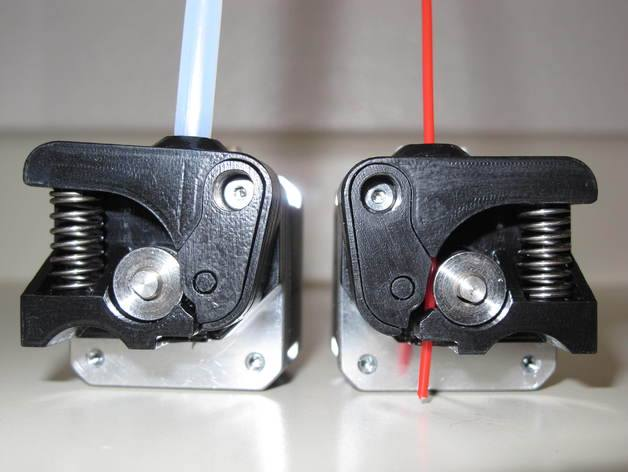
\includegraphics[width=\textwidth,cfbox=azul_marcos 4pt 0pt]{FOTOS/EXTRUSOR3}
		\caption*{\href{http://www.thingiverse.com/thing:403438}{{\footnotesize Printrbot Flexible Filament Direct Drive Extruder by thirdhorizon}}}
    \end{subfigure}
    ~ \qquad %add desired spacing between images, e. g. ~, \quad, \qquad, \hfill etc. 
    %(or a blank line to force the subfigure onto a new line)
    \begin{subfigure}[b]{0.4\textwidth}
        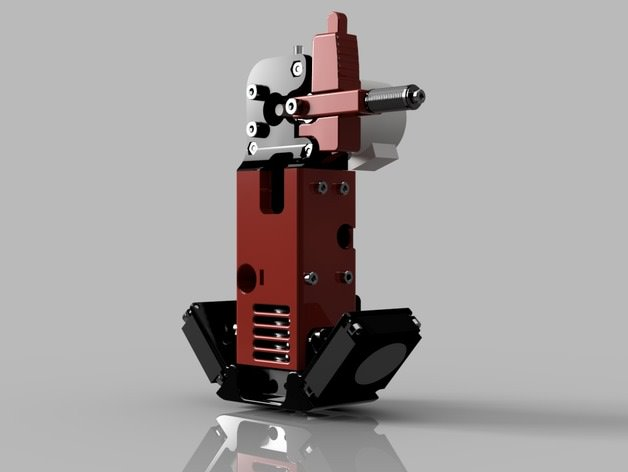
\includegraphics[width=\textwidth,cfbox=azul_marcos 4pt 0pt]{FOTOS/EXTRUSOR4}
		\caption*{\href{http://www.thingiverse.com/thing:1102900}{{\footnotesize Ultimaker 2 PG35L Direct Drive Extruder for 1.75mm E3D v6 Hotend by jasonatepaint}}}
    \end{subfigure}
\end{figure}
			\paragraph{Commercial extruders}\mbox{}\\\\
Acquiring a commercial extruder is more expensive that building one at home, however, they usually perform better than these and they are the best choice when you’re going to use flexible filament intensively.
\\\\
These extruders have been specifically designed to avoid all the problems previously mentioned and some can extrude FlexiSMART at speeds superior to 70 mm/s.
\begin{figure}[H]
    \centering
    \begin{subfigure}[b]{0.4\textwidth}
        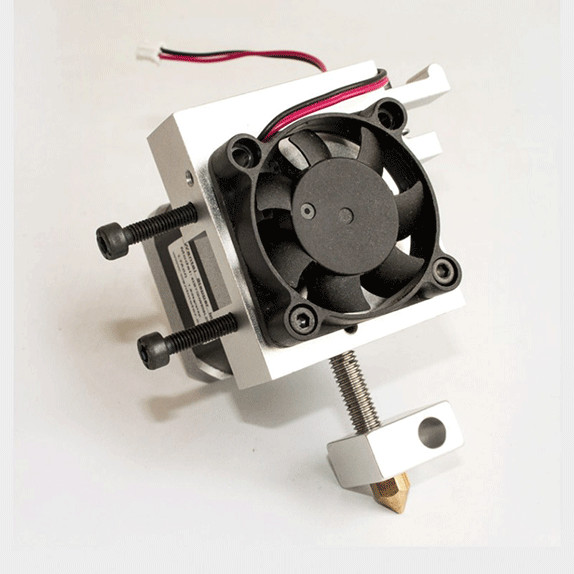
\includegraphics[width=\textwidth,cfbox=azul_marcos 4pt 0pt]{FOTOS/EXTRUSOR5}
		\caption*{\href{http://www.recreus.com}{{\footnotesize Recreus Extruder - Price aprox. 100\euro}}}
    \end{subfigure}
    ~ \qquad%add desired spacing between images, e. g. ~, \quad, \qquad, \hfill etc. 
      %(or a blank line to force the subfigure onto a new line)
    \begin{subfigure}[b]{0.4\textwidth}
        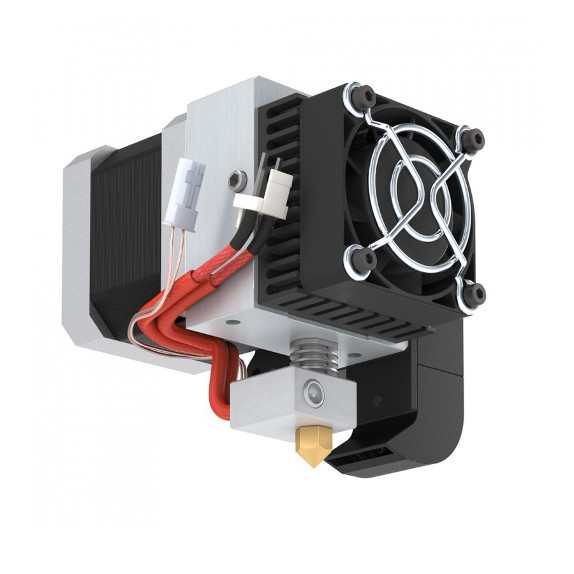
\includegraphics[width=\textwidth,cfbox=azul_marcos 4pt 0pt]{FOTOS/EXTRUSOR6}
		\caption*{\href{http://www.bq.es}{{\footnotesize BQ HeatCore DDG Extruder - Price 140\euro}}}
    \end{subfigure}
\end{figure}
\begin{figure}[H]
    \centering
    ~ %add desired spacing between images, e. g. ~, \quad, \qquad, \hfill etc. 
    %(or a blank line to force the subfigure onto a new line)
    \begin{subfigure}[b]{0.4\textwidth}
        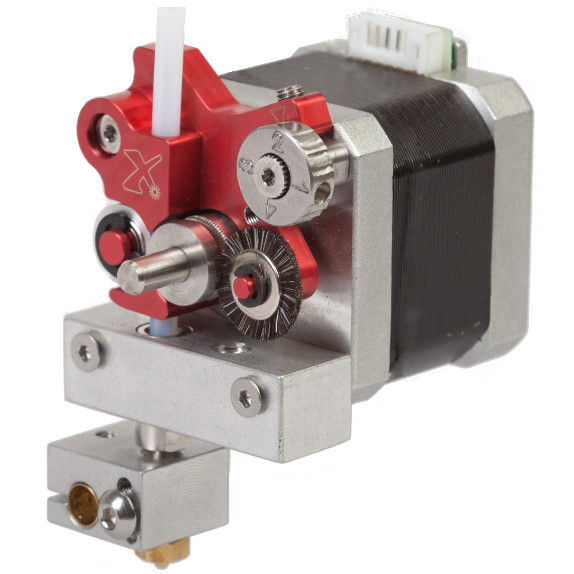
\includegraphics[width=\textwidth,cfbox=azul_marcos 4pt 0pt]{FOTOS/EXTRUSOR7}
		\caption*{\href{https://flexionextruder.com/}{{\footnotesize Flexion Extruder - Price aprox. 140\euro}}}
    \end{subfigure}
    ~ \qquad %add desired spacing between images, e. g. ~, \quad, \qquad, \hfill etc. 
    %(or a blank line to force the subfigure onto a new line)
    \begin{subfigure}[b]{0.4\textwidth}
        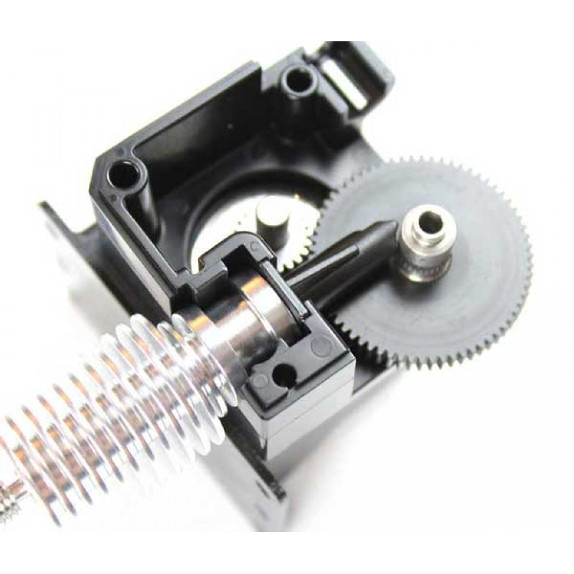
\includegraphics[width=\textwidth,cfbox=azul_marcos 4pt 0pt]{FOTOS/EXTRUSOR8}
		\caption*{\href{www.e3d-online.com}{{\footnotesize Titan Extruder - Price aprox. 70\euro}}}
    \end{subfigure}
\end{figure}
\section{Advices for optimal use of FlexiSMART}
	\subsection{Retraction}
Retraction is a technique used on 3D FFF/FDM printers to improve finishing of the printed parts. It consists on commanding the extruder to retire a few centimeters of filament when this is about to change position to avoid the stringing or apparition of littles threads of filament on different parts of the piece being printed.
\begin{figure}[H]
\centering
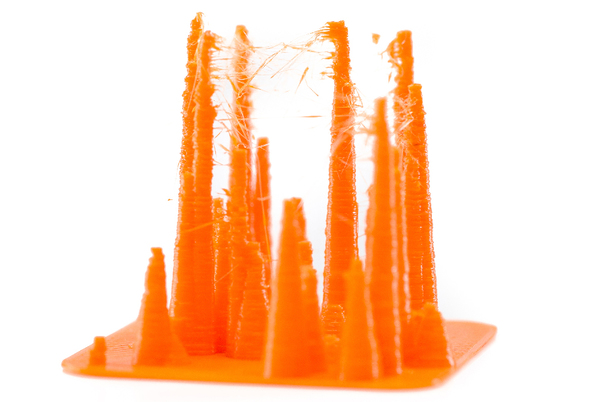
\includegraphics[width=0.5\textwidth,cfbox=azul_marcos 4pt 0pt]{FOTOS/RETRACCION1}
\caption*{A part with stringing problems}
\end{figure}
When using flexible filaments it can happen that by trying to make a very abrupt retraction the filament stretches instead of pulling back. That’s why it’s very recommendable to use retraction parameters different to those used with rigid filaments.
\\\\
The 2 parameters that we can control in the retraction are the size, or lineal amount in millimeters of retracted filament, and the speed on mm/s of the operation. Both values must be inferiors to those used regularly. The optimum way of calibrating these values is to run tests to find out which are the maximum values your printer can take when printing with FlexiSMART. On any case, as a starting point you can use the values recommended by us:
\begin{description}
\item [Retraction size:] 1.5 mm
\item [Retraction speed:] 40 mm/s
\end{description}
Depending on the printer it may be necessary to completely deactivate retraction.
	\subsection{Sequential printing}
FlexiSMART and other flexible filaments have a different viscosity to the one of other materials when it reaches its melting temperature. For this it’s more given to leave small threads of filament between different parts of the piece when the nozzle must move from one point to the other without extruding.
\begin{figure}[H]
\centering
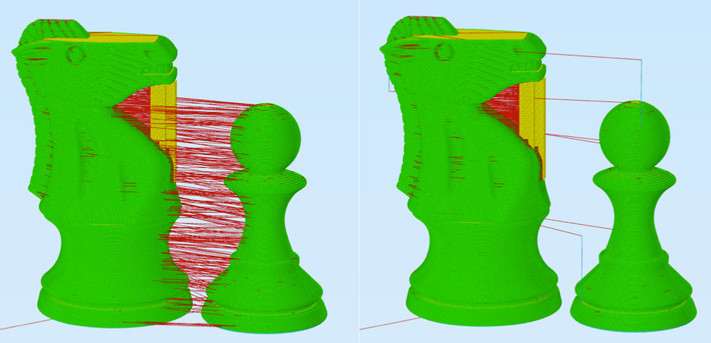
\includegraphics[width=0.5\textwidth,cfbox=azul_marcos 4pt 0pt]{FOTOS/SEQUENTIALPRINTING}
\caption*{Comparison between printing routes of simultaneus and sequential printing}
\end{figure}
Besides, when several parts are going to be printed at the same time, these little threads can appear between the parts since the nozzle has to constantly jump from one to others.
\\\\
As we’ve already previously commented this effect can be reduced by using retraction, but it’s highly recommendable that also the different parts be printed sequentially instead of simultaneously.
\\\\
By sequential printing we mean completely printing a part before starting printing the next.
\\\\
This can be achieved in two different ways:
\begin{itemize}
\item The trivial option is to print only one part and once finished repeat the same print as many times as wanted.
\item The second alternative, more advanced and with some limitations, is to use the laminating option that some programs offer instead of printing one part at a time. The maximum size of the parts that can be printed using this method comes given by the dimensions of the nozzle and the disposition of the axis of the printer. We highly recommend that you get information about how to use the options as not to run the risk of damaging your printer. You can do it through the following links:
\end{itemize}
\url{https://www.simplify3d.com/support/tutorials/multi-part-printing/}\\
\url{http://manual.slic3r.org/advanced/sequential-printing}\\
\url{https://ultimaker.com/en/community/3843-force-cura-to-print-objects-separately}
	\subsection{The first layer}
The first layer is the foundation of the rest of the layers and it can mark the difference between a satisfactory print and a failed print.
\\\\
When printing with FlexiSMART one must pay special attention to the first layer since, at times, a printer correctly leveled to print with PLA or ABS may not be so to print FlexiSMART adequately.
\\\\
To know if the printer is correctly leveled you have to watch attentively how the machine makes the first layer.
\\\\
If the first layer seems translucent it means that the nozzle is too close to the platform and it will be necessary to separate it a few microns.
\\\\
On the other hand, if the first layer seems to detach or the tracks of the deposited material show spaces without plastic between them it will be necessary to bring the nozzle close a few microns to the platform.
\begin{figure}[H]
    \centering
    \begin{subfigure}[b]{0.3\textwidth}
        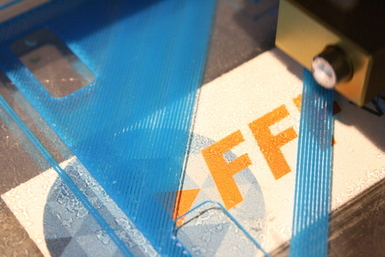
\includegraphics[width=\textwidth,cfbox=azul_marcos 3pt 0pt]{FOTOS/HOTENDALTO}
	\caption*{Nozzle too far}
    \end{subfigure}
    ~ %add desired spacing between images, e. g. ~, \quad, \qquad, \hfill etc. 
      %(or a blank line to force the subfigure onto a new line)
    \begin{subfigure}[b]{0.3\textwidth}
        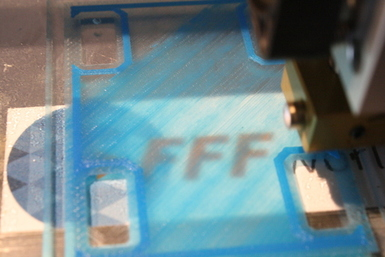
\includegraphics[width=\textwidth,cfbox=azul_marcos 3pt 0pt]{FOTOS/HOTENDBAJO}
	\caption*{Nozzle too close}
    \end{subfigure}
    ~ %add desired spacing between images, e. g. ~, \quad, \qquad, \hfill etc. 
    %(or a blank line to force the subfigure onto a new line)
    \begin{subfigure}[b]{0.3\textwidth}
        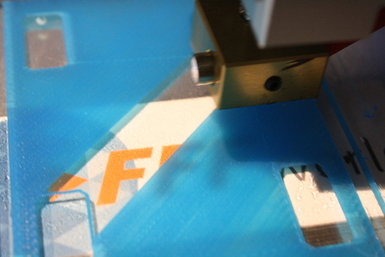
\includegraphics[width=\textwidth,cfbox=azul_marcos 3pt 0pt]{FOTOS/HOTENDPERFECTO}
	\caption*{Nozzle well leveled}
    \end{subfigure}
\end{figure}
This adjustment may be made by software, adjusting the z-offset in the laminated program, or regulating the level mechanism of the printing platform.
	\subsection{Lamination advices}
		\subsubsection{The layer height}
The layer height determines the quality of the part and the printing time.
\\\\
Using a nozzle of 0.4 mm we have proved that the optimal height of the layer is 0.2 mm. With this layer height you will get layers strongly attached with an excellent surface finish.
		\subsubsection{The top layers and perimeters}
The top layers and perimeters are the lateral and superior wrapping of the part. The adequate number of these will depend on the infill and the use given to the part.
\\\\
With a high infill, you can reduce the top-layers number to 3 since the filling of the part will give them a good base to stand on. Using some medium or low values of infill is recommendable to rise the number of top-layers to 5 to make sure that the top of the part is completely sealed.
\\\\
If the part is going to suffer deformations it is recommendable to rise the number of shells or horizontal perimeters. Rising the number of horizontal perimeters will stop the walls of the part to quarter when exerting pressure or traction on them.
\\\\
These recommendations are valid when you use a nozzle of 0.4 mm and a layer height of 0.2 mm. if the size of the nozzle or the layer varies, the number of perimeters and optimal top-layers will also change.
\\\\
We invite you to run your own tests and share the results with us.
		\subsubsection{Influence of the infill in flexibility}
The amount and design of the infill has a great influence on the degree of flexibility of the parts printed with FlexiSMART.
\\\\
A part with infill close to 100\% will behave as a rubber block and can be a good choice for parts such as silent-blocks or spacers.
\\\\
Using an infill of 15\% you’ll get soft parts that could be crushed and deformed.
\\\\
The infill pattern also affects the flexibility and a rectilinear infill doesn’t behave the same as a honeycomb infill. We invite you to make your own tests and choose the one that suits your project the most.
	\subsection{Use of a greater size nozzle}
The standard nozzle of the most of the printers has 0.4 mm, a nozzle size that gives a good speed/resolution ratio. FlexiSMART is perfectly printed with this type of nozzle, however it is convenient to make some clarifications.
\\\\
The size of the nozzle limits the amount of material that can be extruded per unit of time. By using rigid filaments this limit is higher since the speed can be increased and the filament itself supports the necessary extra pressure for the material to exit by the nozzle. With FlexiSMART however, the filament is compressed if this pressure is too high and, in general, it must be printed at lower speeds.
\\\\
Therefore if you want to extrude FlexiSMART at high speeds it is recommendable that you use a nozzle of bigger size, from 0.6 mm. Using one of these nozzle you could print a lot quicker, with superior layer heights, sacrificing some resolution.
\section{Would you like to support our project?}
All the members of FFF World love 3D printing and the maker community. We feel lucky to be able to work on projects where we can deliver our honest passion. In the future, we would like to be able to develop more materials, more colors and more formats. Ultimately, we would like to be able to make our company grow.
\\\\
Therefore, one of the best actions to help us, if you want to do it and you’re satisfied with the filament, is to give us a 5 stars rating on amazon.
\begin{figure}[H]
\centering

\includegraphics[width=0.5\textwidth,cfbox=azul_marcos 1pt 0pt]{FOTOS/AMAZON_FIVE_STARS}
\caption*{Thanks a lot!}
\end{figure}
\subsection{Other filaments with awesome properties available today in Amazon}
\begin{description}
\item[FlexiSMART Tech:] Designed to resist the abrasion and wear of technical printings.
\item[ABS Tech:] Minimized warping effect. High performance on technical applications.
\item[PETG Tech:] Maximum mechanical resistance. Resistant to contact with water and UV rays. Apt for alimentary use.
\item[FilaMETAL:] PLA with non-abrasive metallic charge that gives a spectacular mechanical finish to your printings.
\item[PC Tech:] Polycarbonates with a high resistance to temperature and excellent mechanic properties.
\item[Nylon Tech:] printable at low temperature. Resistance to bangs with a certain degree of flexibility.
\item[PVA Tech:] Water soluble filament indicated for use as support material. Excellent compatibility with PLA.
\item[HIPS Tech:] Limonene soluble filament indicated for use as support material. Good mechanical resistance and excellent compatibility with ABS.
\end{description}
%\section{Bibliografía}
%Esta guía no habría sido posible sin el conocimiento libre generado por la comunidad RepRap. Para la elaboración de esta guía se han %utilizado imágenes y contenido extraidos de los siguientes sitios web.
%\\\\
%\url{http://www.gyrobot.co.uk/blog/how-to-3d-print-with-flexible-filaments}\\
%\url{http://www.thingiverse.com/thing:1496895}\\
%\url{http://www.thingiverse.com/thing:247024}\\
%\url{http://www.thingiverse.com/thing:16319}\\
%\url{http://www.thingiverse.com/thing:779011}\\
%\url{http://www.thingiverse.com/thing:1102900}\\
%\url{http://www.thingiverse.com/thing:147705}\\
%\url{http://www.thingiverse.com/thing:222667}\\
%\url{http://www.thingiverse.com/thing:512338}\\
%\url{https://all3dp.com/common-3d-printing-problems-and-their-solutions/}\\
%\url{https://www.simplify3d.com/support/}\\
%\url{http://www.thingiverse.com/thing:508896}\\
%\url{http://www.thingiverse.com/thing:1187344}

\includepdf{PDF/EN_CONTRAPORTADA.pdf}
\end{document}
